\documentclass[12pt]{article}
\usepackage[margin=0.5in]{geometry}
\usepackage{amssymb}
\usepackage{amsmath}
\usepackage{enumitem}
\usepackage{graphicx}
\usepackage{float}
% Create Real, Complex, Integer sets, and principal arg command
\newcommand{\real}{\mathbb{R}}
\newcommand{\complex}{\mathbb{C}}
\newcommand{\integer}{\mathbb{Z}}
\newcommand{\Arg}{\operatorname{Arg}}
\newcommand{\mightequal}{\stackrel{?}{=}}
% Use Re and Im for real and imaginary operators
\renewcommand{\Re}{\operatorname{Re}}
\renewcommand{\Im}{\operatorname{Im}}
\graphicspath{{images/}}
\begin{document}
\normalsize
\section {Abstract}
This document is the study guide for Nathaniel Barlow's Complex Variables examination on 13 December 2018.  It was written by Ryan Volz using materials given in class.

The examination consists of twelve topics, each of which are detailed in this study guide.  Each topic includes a bulleted list of required knowledge followed by an example problem as given in class.

In this document, the imaginary number is referred to as $i$, and a complex number $z$ has real part $a$ and imaginary part $b$.

\section{Topic 1: Sketching a Curve in the Complex Plane}
\subsection{Required Knowledge}
\begin{itemize}
    \item The imaginary number, referred in this course as $i$, is defined as $i=\sqrt{-1}$.  Thus, $i^2=-1$.
    \item The domain of complex numbers is defined as any number which can be expressed as $a+bi$, where both $a$ and $b$ are real.
    \item For $z=a+bi$ ($a\in\real, b\in\real$), $a=\Re[z]$ (a is the real part of z) and $b=\Im[z]$ (b is the imaginary part of z).
\end{itemize}
\subsection{Problem}
\textit{Note: This problem uses knowledge from Topic 2 (Section \ref{Topic 2: Complex Arithmetic}), as it is difficult to construct a meaningful problem with just the information given.}
Sketch the graph of $z\in\complex$ in the complex plane, where:
$|z-2i|=\Im[z]$
\subsection{Solution}
Let $a=\Re[z], b=\Im[z]$.

\begin{equation}
	|z-2i|=b
\end{equation}
\begin{equation}
	|a+ib-2i|=b
\end{equation}
\begin{equation}
	|a+i(b-2)|=b
\end{equation}
\begin{equation}
	\sqrt{a^2+(b-2)^2}=b
\end{equation}
\begin{equation}
	a^2+(b-2)^2=b^2
\end{equation}
\begin{equation}
	a^2+b^2-4b+4=b^2
\end{equation}
\begin{equation}
	a^2+4=4b
\end{equation}
\begin{equation}
	4b=a^2+4
\end{equation}
\begin{equation}
	b=\frac{a^2}{4}+1
\end{equation}

This is the equation of a parabola.  The graph is below.
\begin{figure}[H]
    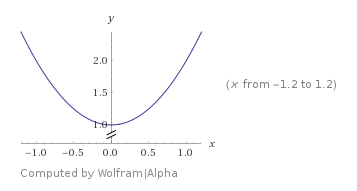
\includegraphics{Topic1Graph.png}
\end{figure}

\section{Topic 2: Complex Arithmetic}
\subsection{Required Knowledge}
\begin{itemize}
    \item $|z|$, or the modulus of $z$, is the distance from zero.  Thus $|a+bi|=\sqrt{a^2+b^2}$.
    \item $\arg(z)$ is an angle that the complex number forms with the positive real ray.  Thus, $\arg(z)$ can result in an infinite number of angles (each offset by $2\pi$).
    \item $\Arg(z)$ is the smallest possible angle that the complex number forms with the positive real ray.
    \item In the case that a z is negative and real, $Arg(z)$ is considered to be $\pi$.  Thus, for any $z\in\complex$, $-\pi<Arg(z)<\pi$.
    \item Euler's Identity states that for any $z\in\complex$, $z=re^{i\theta}$ where $\theta=arg(z), r=|z|$.  This form is called polar form.
    \item $|e^z|=e^{\Re[z]}$ and $\arg(e^z)=\Im[z]+2k\pi (k\in\real)$
    \item Cosine Identities: $\cos(z)=\Re[e^iz]=\frac{e^{iz}+e^{-iz}}{2}$
    \item Sine Identities: $\sin(z)=\Im[e^iz]=\frac{e^{iz}-e^{-iz}}{2i}$
\end{itemize}
\subsection{Problem}
Let $z=2\pi-2\pi i$.
\begin{enumerate}[label=\alph*. ]
    \item Plot $z$ in the complex plane.
    \item Compute $|z|$.
    \item Write $z$ in polar form.
    \item Compute $e^z$.
    \item Compute $\arg(e^z)$.
    \item Evaluate $\cos(z)$.
\end{enumerate}
\subsection{Solution (a)}
The graph is included below.
\begin{figure}[H]
    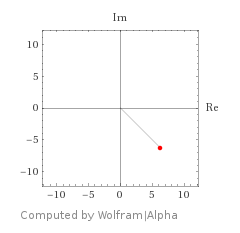
\includegraphics{Topic2Graph.png}
\end{figure}
\subsection{Solution (b)}
\begin{equation}
	|z|=\sqrt{(\Re[z])^2+(\Im[z])^2}
\end{equation}
\begin{equation}
	|z|=\sqrt{(2\pi)^2+(2\pi)^2}
\end{equation}
\begin{equation}
	=\sqrt{4\pi^2+4\pi^2}
\end{equation}
\begin{equation}
	=\sqrt{8\pi^2}
\end{equation}
\begin{equation}
	=c\sqrt{2}\pi
\end{equation}
\subsection{Solution (c)}
Use the unit circle provided on the examination to solve this problem.
\begin{equation}
	arg(z)=\frac{-\pi}{4}
\end{equation}
\subsection{Solution (d)}
Use the solutions from (b) and (c) along with Euler's Identity.

\begin{equation}
	z=re^{i\theta}
\end{equation}
\begin{equation}
	z=|z|e^{iarg(z)}
\end{equation}
\begin{equation}
	z=2\sqrt{2}\pi e^{\frac{-i\pi}{4}}
\end{equation}

As the problem only asked for one solution, we could have used any solution for $\arg(z)$.
\subsection{Solution (e)}

\begin{equation}
	|e^z|=e^{\Re[z]}=e^{2\pi}
\end{equation}
\subsection{Solution (f)}

\begin{equation}
	\arg(e^z)=\Im[z]+2k\pi,\:k\in\integer
\end{equation}
\subsection{Solution (g)}

\begin{equation}
	\cos(z)=\frac{e^{iz}+e^{-iz}}{2}
\end{equation}
\begin{equation}
	=\frac{e^{i(2\pi-2\pi i)}+e^{-i(2\pi-2\pi i)}}{2}
\end{equation}
\begin{equation}
	=\frac{e^{2\pi i}e^{2\pi}+e^{-2\pi i}e^{-2\pi}}{2}
\end{equation}
\begin{equation}
	=\frac{e^{2\pi}+e^{-2\pi}}{2}
\end{equation}
\section{Topic 3: Raising a Complex Number to an Integral Power}
\subsection{Required Knowledge}
\begin{itemize}
    \item In order to raise a complex number to an integral power, convert the complex number to polar form and distribute the exponent to both the coefficient and the power on $e$.
    \item For raising to an integral power, any argument for the polar form may be chosen (typically this is the principal argument).
    \item In order to rationalize the denominator of a complex fraction, multiply the top and bottom of the fraction by the complex conjugate of the denominator ($a-bi$)
\end{itemize}

\subsection{Problem}

Evaluate the following and put the result in the form $a+bi$:

\begin{equation}
	z=(\frac{-i}{1+i})^{13}
\end{equation}
\subsection{Solution}

\begin{equation}
	z=(\frac{-i}{1+i}*\frac{1-i}{1-i})^{13}
\end{equation}
\begin{equation}
	=(\frac{-1-i}{2})^{13}
\end{equation}
\begin{equation}
	=(-\frac{1}{2}-\frac{1}{2}i)^{13}
\end{equation}
\begin{equation}
	=(2^{-\frac{1}{2}}e^{\frac{-3\pi}{4}i})^{13}
\end{equation}
\begin{equation}
	=2^{-\frac{13}{2}}e^{\frac{-39\pi}{4}i}
\end{equation}
\begin{equation}
	=2^{-8}\sqrt{2}e^{\frac{-\pi}{4}i}
\end{equation}
\begin{equation}
	=\frac{\sqrt{2}}{128}(\cos(\frac{\pi}{4})+i\sin(\frac{\pi}{4}))
\end{equation}
\begin{equation}
	=\frac{\sqrt{2}}{128}(\frac{1}{\sqrt{2}}+i\frac{1}{\sqrt{2}})
\end{equation}
\begin{equation}
	=\frac{1}{128}(1+i)
\end{equation}
\begin{equation}
	=\frac{1}{128}+\frac{1}{128}i
\end{equation}
\section{Topic 4: Raising a Complex Number to a Rational Power}
\subsection{Required Knowledge}
\begin{itemize}
    \item In order to raise a complex number to a rational power, follow the same steps as an integral power.
    \item However, the general form for $\arg(z)$ must be used, adding $2k\pi i$ to the principal argument, and solve for any $k$.
    \item The number of roots will be equal to the denominator of the exponent when it is fully reduced (unless the radius is zero, in which case there is only one distinct root).
    \item In order to find all roots, enumerate $k$ (starting at any point) unil the required number of roots are found.
\end{itemize}

\subsection{Problem}

Solve for all roots of z and put the result in the form $a+bi$:

\begin{equation}
	z^3=-125
\end{equation}
\subsection{Solution}
Let $k\in\integer$.
\begin{equation}
	z^3=125e^i(\pi+2k\pi)
\end{equation}
\begin{equation}
	z=125^{\frac{1}{3}}e^i(\frac{\pi+2k}{3})
\end{equation}
\begin{equation}
	z=5e^i(\frac{\pi+2k}{3})
\end{equation}

There are three roots, which we will call $z_0$, $z_1$, $z_2$.  $z_0$ will be found when $k=0$, $z_1$ when $k=1$, and $z_2$ when $k=3$.
\begin{equation}
	z_0=5e^{i\frac{\pi}{3}}
\end{equation}
\begin{equation}
	z_0=5(\cos(\frac{\pi}{3})+i\sin(\frac{\pi}{3}))
\end{equation}
\begin{equation}
	z_0=5(\frac{\sqrt{3}}{2}+\frac{1}{2}i)
\end{equation}
\begin{equation}
	z_0=\frac{5\sqrt{3}}{2}+\frac{5}{2}i
\end{equation}
\begin{equation}
	z_1=5e^{i\pi}
\end{equation}
\begin{equation}
	z_1=5(\cos(\pi)+i\sin(\pi))
\end{equation}
\begin{equation}
	z_1=5(-1+0i)
\end{equation}
\begin{equation}
	z_1=-5
\end{equation}
\begin{equation}
	z_2=5e^{i\frac{4\pi}{3}}
\end{equation}
\begin{equation}
	z_2=5(\cos(\frac{4\pi}{3})+i\sin(\frac{4\pi}{3}))
\end{equation}
\begin{equation}
	z_2=5(\frac{-\sqrt{3}}{2}+\frac{1}{2}i)
\end{equation}
\begin{equation}
	z_2=\frac{-5\sqrt{3}}{2}+\frac{5}{2}i
\end{equation}
\begin{equation}
	z\in\{\frac{5\sqrt{3}}{2}+\frac{5}{2}i,-5,\frac{-5\sqrt{3}}{2}+\frac{5}{2}i\}
\end{equation}

\section{Topic 5: Differentiability of a Complex Function}
\textit{Note: Originally, Topic 5 was "Finding the Limits of a Complex Function", however, this has been removed from the examination.}

\subsection{Required Knowledge}
\begin{itemize}
    \item The Cauchy\-Riemann equations for a function $z=u(x,y)+iv(x,y)$ are $\frac{\partial u}{\partial x}=\frac{\partial v}{\partial y}$ and $\frac{\partial v}{\partial x}=-\frac{\partial u}{\partial y}$
    \item A complex function is differentiable in the complex plane if and only if the Cauchy\-Riemann equations hold for it.
    \item If the Cauchy\-Riemann equations hold, the complex derivative of a function $f(z)$ is $f\prime(z)=\frac{\partial u}{\partial x}+i\frac{\partial v}{\partial x}=\frac{\partial v}{\partial y}-i\frac{\partial y}{\partial y}$.
\end{itemize}
\subsection{Problem}
Determine whether the complex derivative of $f(x,y)=x+ix^2$ exists.  If it exists, find the derivative.
\subsection{Solution}
First, solve for the partial derivatives.

\begin{equation}
	\frac{\partial u}{\partial x}=1
\end{equation}
\begin{equation}
	\frac{\partial v}{\partial x}=2x
\end{equation}
\begin{equation}
	\frac{\partial u}{\partial y}=0
\end{equation}
\begin{equation}
	\frac{\partial v}{\partial y}=0
\end{equation}

Check that the Cauchy\-Riemann equations hold:
\begin{equation}
    \frac{\partial u}{\partial x}\mightequal\frac{\partial v}{\partial y}\;\&\;\frac{\partial v}{\partial x}\mightequal-\frac{\partial u}{\partial y}
\end{equation}
\begin{equation}
    1\mightequal0\;\&\;2x\mightequal-0
\end{equation}
These equations hold nowhere.  Thus, the function is not differential anywhere.  However, we can attempt to calculate the derivative using the derivative equations:

\begin{equation}
    f\prime(z)=\frac{\partial u}{\partial x}+i\frac{\partial v}{\partial x}=\frac{\partial v}{\partial y}-i\frac{\partial u}{\partial y}
\end{equation}
\begin{equation}
    =1+2xi=0
\end{equation}
The two equations do not agree.  This is a consequence of the Cauchy\-Riemann equations not holding.

\section{Topic 6: Finding roots using complex logarithms}
\subsection{Required Knowledge}
\begin{itemize}
    \item In this course, the real logarithm function is specified as $\log_e(x)$ to prevent a self-reference when defining the complex logarithm function.
    \item The complex logarithm function $\ln(z)$ is defined as $\log_e(|z|)+iarg(z)$.
\end{itemize}
\subsection{Problem}
Solve for all roots of z, where:

\begin{equation}
    e^{iz}=3+3i
\end{equation}
\subsection{Solution}
Let $k\in\integer$
\begin{equation}
    \ln(e^{iz})=\ln(3+3i)
\end{equation}
\begin{equation}
    iz=\ln(3+3i)
\end{equation}
\begin{equation}
    iz=\log_e(|3+3i|)+i\arg(3+3i)
\end{equation}
\begin{equation}
    iz=\log_e(3\sqrt{2})+i(\frac{\pi}{4}+2k\pi)
\end{equation}
\begin{equation}
    z=-i\log_e(3\sqrt{2})+\frac{\pi}{4}+2k\pi
\end{equation}
\begin{equation}
    z=\frac{\pi}{4}+2k\pi-i(\log_e{3}+\frac{1}{2}\log_e{2})
\end{equation}
\section{Topic 7: Using the parametric circle formula to solve a complex integral}
\subsection{Required Knowledge}
\begin{itemize}
    \item For an integral $\int_{C}{f(z)dz}$, the integral of $f(z)$ along the circular arc $C$, replace $z$ with $z_0+re^{i\theta}$ ($z_0$ being the centre), and $C$ with $\theta$, from 0 to the final angle.
\end{itemize}
\subsection{Problem}
Solve the following integral:
\begin{equation}
    \int_C{\frac{1}{\Re[z]}}dz
\end{equation}

Where $C$ is the circular arc centred at the origin with a radius of 2 from $\theta=0$ to $\theta=\frac{\pi}{4}$.
\subsection{Solution}
Replace $z$ with its polar form, $z=z_0+re^{i\theta}$.  In this case, $z_0=0$ as it is centred at the origin, and $r=2$, thus $z=2e^{i\theta}$, and $dz=2ie^{i\theta}dt$.  $\theta$ is the path of integration, from $0$ to $\frac{\pi}{4}$.
\begin{equation}
    \int_0^{\frac{\pi}{4}}{\frac{1}{\Re[2e^{i\theta}]}2ie^{i\theta}}d\theta
\end{equation}\begin{equation}
    \int_0^{\frac{\pi}{4}}{\frac{1}{2\Re[e^{i\theta}]}2ie^{i\theta}}d\theta
\end{equation}
\begin{equation}
    \int_0^{\frac{\pi}{4}}{\frac{1}{\Re[e^{i\theta}]}ie^{i\theta}}d\theta
\end{equation}
\begin{equation}
	\int_0^{\frac{\pi}{4}}{\frac{ie^{i\theta}}{\Re[e^{i\theta}]}}d\theta
\end{equation}
\begin{equation}
    \int_0^{\frac{\pi}{4}}{\frac{i\cos(\theta)-\sin(\theta)}{\cos(\theta)}}d\theta
\end{equation}
\begin{equation}
    \int_0^{\frac{\pi}{4}}(i-\tan(\theta))d\theta
\end{equation}
\begin{equation}
	[i\theta + \ln(\cos(\theta))]_0^{\frac{\pi}{4}}
\end{equation}
\begin{equation}
	\frac{\pi}{4}i-0i+\ln(\cos(\frac{\pi}{4}))-\ln(\cos(0))
\end{equation}
\begin{equation}
	\frac{\pi}{4}i+\ln(2^{-\frac{1}{2}})-\ln(1)
\end{equation}
\begin{equation}
	\frac{\pi}{4}i-\frac{1}{2}\ln(2)-0
\end{equation}
\begin{equation}
	-\frac{1}{2}\ln(2)+\frac{\pi}{4}i
\end{equation}
\end{document}